\chapter{Overview}\label{ch:overview}

\section{Purpose of the system}

The system calculates the drag coefficient $C_D$ of the Aconcagua rocket as a
function of the Mach number with OpenFOAM v2412. The output of record is the
curve $C_D(M)$ at $M = 0.3$, $0.6$, $0.8$, $1.2$ and $1.8$, at angles of attack
$\alpha = 0^\circ$, $4^\circ$ and $8^\circ$, on three meshes for a mesh-convergence
study. The flight conditions are those of the coast phase of the IREC flight in
Midland (\cref{sec:flight-conditions}).

The mesh must resolve these flow features, in this order of priority:

\begin{enumerate}
\item The shock waves, for $M \geq 0.8$.
\item The base wake. The base drag is a large part of the drag of a rocket.
\item The wall friction. It depends on \yplus.
\end{enumerate}

The tip vortex of the fins is not a priority. Do not add cells for it.

\section{Process}

\Cref{fig:process} shows the process. Each step is a script, and each script
has a section in this guide.

\begin{figure}[htbp]
  \centering
  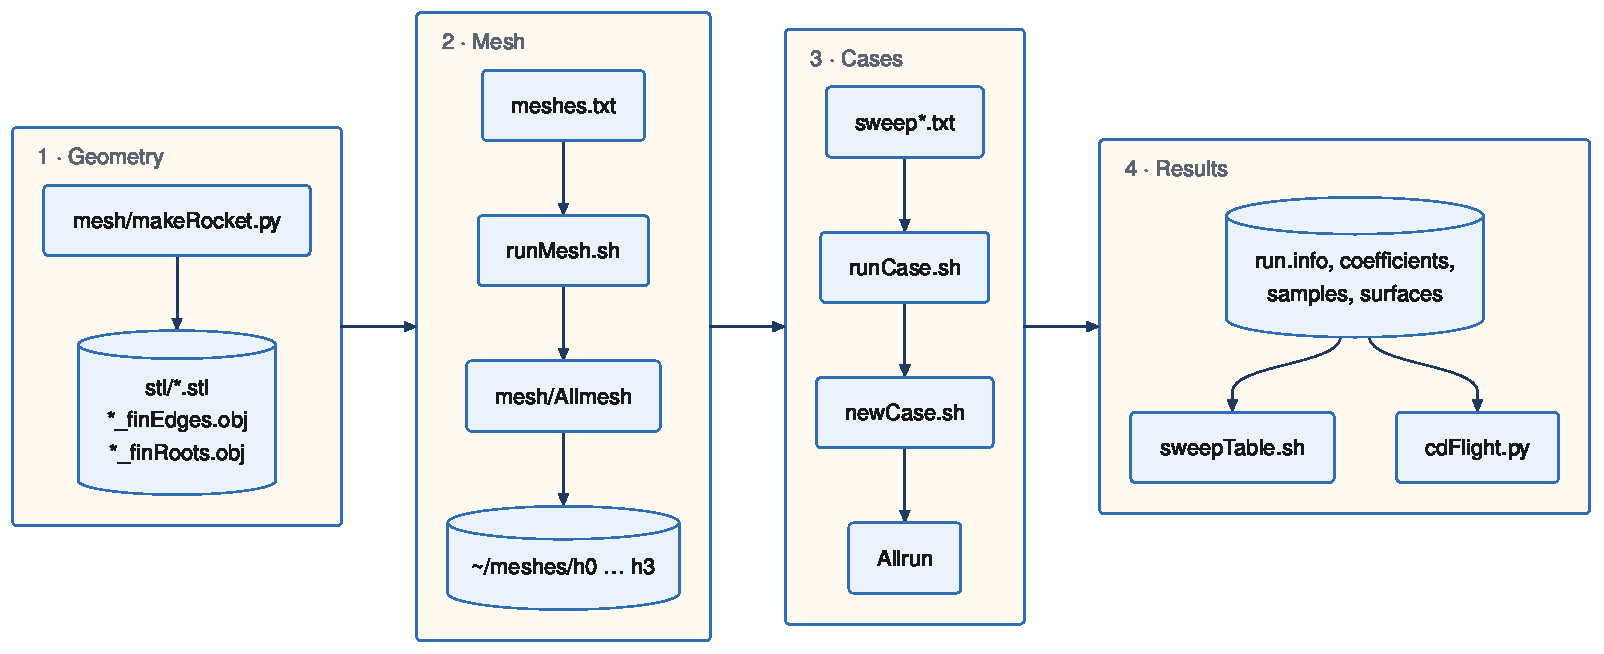
\includegraphics[width=\linewidth]{figures/pdf/process.pdf}
  \caption{Process from the geometry to the results.}
  \label{fig:process}
\end{figure}

\begin{steps}
\item \file{mesh/makeRocket.py} writes the geometry as an STL file and two edge
  files (\cref{ch:geometry}).
\item \file{mesh/Allmesh} makes one mesh. \file{runMesh.sh} makes all the meshes of
  \file{meshes.txt} (\cref{ch:mesh,sec:run-mesh}).
\item \file{newCase.sh} makes one case from a template, a mesh and a flight
  condition. \file{common/Allrun} runs it (\cref{ch:cases}). \file{runCase.sh}
  does the two steps for each line of a sweep file (\cref{ch:sweeps}).
\item Each run writes its coefficients, its samples and a record of the machine
  (\cref{ch:results}). \file{post/sweepTable.sh} collects a sweep in one table, and
  \file{flightData/cdFlight.py} compares it with the flight (\cref{ch:flight}).
\end{steps}

\section{Two solvers}

The case templates use two solvers, with the change at $M = 1$:

\begin{tabularx}{\linewidth}{@{}l l L@{}}
\toprule
Template & Solver & Use \\
\midrule
\file{case-pimple/} & \cmd{rhoPimpleFoam} & $M < 1$, and the first run of each $M > 1$ chain \\
\file{case-central/} & \cmd{rhoCentralFoam} & $M > 1$ \\
\bottomrule
\end{tabularx}

\medskip
\Cref{ch:solvers} gives the reasons and the models.

\section{Directory structure}

\begin{longtable}{@{}P{0.36\linewidth} P{0.58\linewidth}@{}}
\caption{Contents of \texttt{flightModel/}.}\label{tab:dirs}\\
\toprule
Path & Contents \\
\midrule
\endfirsthead
\toprule
Path & Contents \\
\midrule
\endhead
\file{mesh/makeRocket.py} & Writes the geometry: the STL file and its edge files (\cref{sec:makerocket}). \\
\file{mesh/stl/} & The geometry files. \file{Aconcagua_biconvex117_roll45.stl} is the default (fins at $45^\circ$). \\
\file{mesh/Allmesh} & Makes one mesh (\cref{sec:allmesh}). \\
\file{mesh/snapPlane.py} & Sets $z = 0$ on the cut of a half mesh. \\
\file{mesh/system/} & \file{meshDict}, \file{createPatchDict}, \file{createPatchDictHalf}, \file{topoSetDictHalf}, and the dictionaries that the mesh applications need. \\
\file{mesh/meshInfo} & Reference values and fin geometry of the mesh (\cref{sec:meshinfo}). \\
\file{case-central/} & Template for \cmd{rhoCentralFoam}. It also holds the files that the two templates share. \\
\file{case-pimple/} & Template for \cmd{rhoPimpleFoam}. It holds only the files that differ. \\
\file{common/Allrun}, \file{common/Allrefine}, \file{common/machineLog.py} & Scripts that \file{newCase.sh} copies into each case. \\
\file{newCase.sh} & Makes one case (\cref{sec:make-case}). \\
\file{runMesh.sh}, \file{meshes.txt} & Make the meshes of the sweep (\cref{sec:run-mesh}). \\
\file{runCase.sh}, \file{sweep*.txt} & Make and run the cases of a sweep (\cref{sec:run-sweep}). \\
\file{post/monitor.sh} & Plots a run while it runs (\cref{sec:monitor}). \\
\file{post/sweepTable.sh} & Writes a sweep as a CSV table (\cref{sec:sweeptable}). \\
\file{post/firstLayer.py} & Measures the first cell on the walls of a mesh (\cref{sec:layers}). \\
\file{flightData/} & The TeleMega data of the flight and \file{cdFlight.py} (\cref{ch:flight}). \\
\file{docs/guide/} & This guide. \\
\bottomrule
\end{longtable}

\section{Computers}\label{sec:computers}

\begin{tabularx}{\linewidth}{@{}l L L@{}}
\toprule
 & \texttt{newton} & \texttt{nemepad} \\
\midrule
CPU & 2 $\times$ Xeon E5-2660 v4, 2 sockets of 14 cores & Ryzen 7 250, 1 socket of 8 cores, 16 threads \\
Memory & ECC & \unit{28}{GB}, no ECC \\
Open MPI & 4.1 & 5.0.10 \\
Locale & \texttt{es\_ES}: \cmd{awk} writes decimal commas (\cref{sec:ts-locale}) & \texttt{en} \\
Sweep files & \file{sweepSubsonic.txt}, \file{sweepSupersonic.txt}, one on each socket & \file{*.nemepad.txt}, one file at a time \\
Status (2026-10-18) & Out of service: the memory module DIMM\_A1 stops the computer under load & In use \\
\bottomrule
\end{tabularx}
